\documentclass{standalone}

\usepackage{tikz}
\usepackage{pgfplots}
\usetikzlibrary{calc}
\pgfplotsset{compat=1.15}

\begin{document}

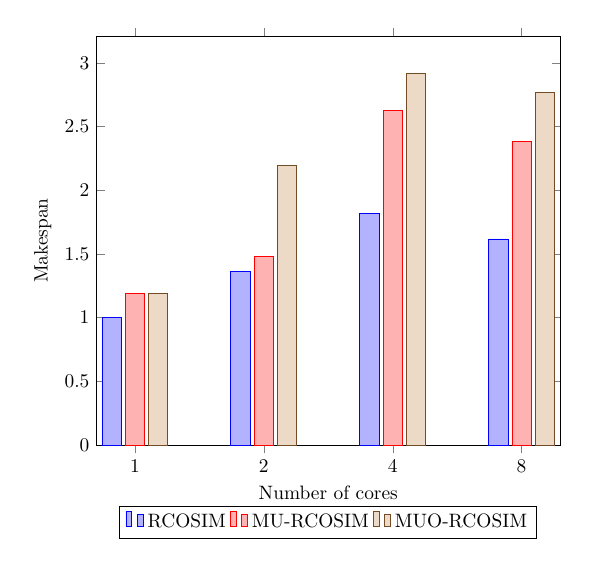
\begin{tikzpicture}[scale=0.7]
    \begin{axis}[
        height=9cm,
        width=10cm,
       % x tick label style={/pgf/number format/1000 sep=},
				symbolic x  coords={1,2,4,8},
        xlabel=Number of cores,
				ylabel=Makespan,
				ymin=0,
        %enlargelimits=0.15,
        legend style={at={(0.5,-0.15)},
        anchor=north,legend columns=-1},
        ybar,
				xtick={1,2,4,8},
        bar width=10pt,
        ]
        
				\addplot
        coordinates {
				  (1,	1)
					(2,	1.36054707312381)
					(4,	1.81769750216137)
					(8,	1.61759996672974)
				};
        
				\addplot
        coordinates {
				(1,	1.18980759230369)
				(2,	1.48243006326702)
				(4,	2.62491564313673)
				(8,	2.38369848322353)
				  
				};
				
				\addplot
        coordinates {
				  (1,	1.18980759230369)
					(2,	2.1954055426991)
					(4,	2.91792948237059)
					(8,	2.76770911160921)
				};
			
        
        \legend{RCOSIM,MU-RCOSIM,MUO-RCOSIM}
    \end{axis}
\end{tikzpicture}

\end{document}